\chapter{Conclusion}
\label{conclusion}

\section{Research Question Revisited}

This section revisted the three research questions defined in Chapter 1.


\textbf{Research Question 1: }\textit{What are the challenges in search-based crash reproduction?}

With this research question, we tried to detect and categorize the challenges in search-based crash reproduction. Since previous evaluations of these techniques contained a limited number of subjects (at most 50 cases), we could not conclude a concrete answer from these experiments' results. Hence, to take the first step towards answering this research question, we designed a benchmark, called \crashpack, which includes 200 real-world Java crashes. We also proposed a new tool, called \exrunner, to conduct extensive experiments on these crashes.

We made both \crashpack and \exrunner publicly available for two purposes: 
(i) ease the comparison of the existing crash reproduction techniques against the existing ones for other researchers in the community of automated crash reproduction; and 
(ii) help researchers to identify the impacting factors, which makes the different outcomes for each crash reproduction technique.

We utilized \exrunner to apply the state of the art automated crash reproduction tool (\evocrash) on all crashes in \jcrashpack. The outcome of this experiment shows that \evocrash is not successful in reproducing more than 50\% of the crashes in \jcrashpack. Hence, we performed an extensive manual analysis to identify the challenges leading to unsuccessful crash reproduction in this search-based approach. We characterized the identified challenges into 13 categories. Some of the identified challenges (\eg complex input generation, complex code, \etc) are related to general search-based test generation issues.

This research question confirms that there is still space for improvements in search-based crash reproduction and test generation techniques, despite their undeniable achievements. For instance, since some of the challenges identified in this research question (complex input data generation and complex code) are indicating the complexity of the problem in search-based crash reproduction and test generation, we settle that using pure randomness, without using any other sources of information, is not enough for the search process to generate complex solutions.



\textbf{Research Question 2: }\textit{Based on the identified challenges, how can we leverage the existing knowl\-edge, carved from information sources, to steer the crash reproduction search process?}


With this research question, we sought to address two of the most common challenges in search-based crash reproduction, which identified in Research Question 1: Input Data Generation, and Complex Code. For this purpose, this thesis introduced new techniques and search objectives, which utilize the pieces of knowledge carved from different information sources such as source code and manually-written tests.

In Chapter \ref{sec:model_seeding}, we introduced a new seeding technique for search-based crash reproduction, called behavioral model seeding, to address complex input data generation challenge. This seeding strategy monitors and abstracts the usages of objects in source code and existing test suites. Then, it uses these models to generate test cases during the search process.
We assessed the relevance of using this seeding strategy in search-based crash reproduction. We also compared the behavioral model seeding with the state-of-the-art seeding strategy (called test seeding), which only seeds the existing test cases to the search process. We witnessed that behavioral model seeding outperforms search-based crash reproduction without seeding and with test seeding in terms of effectiveness and efficiency. These results indicate that behavioral model seeding improves the search process in crash reproduction to tackle the complex input data generation issue, identified in Research Question 1, in more cases.

Chapter \ref{sec:moho:introduction} introduces a novel technique (called \moho), which combines different information sources to improve the exploration ability of the search process in crash reproduction. Improving the exploration in this search-based technique leads to more diverse test cases during the search process. By generating more diverse test cases, the search process can generate more complex solutions with more complex input data \cite{jensen2004helper}. The results presented in this chapter show that using multiple information sources to define new helper objectives for crash reproduction improves search-based crash reproduction in terms of effectiveness and efficiency.

Finally, Chapter \ref{section:bbc:introduction} addresses the complex code challenge, which is identified in Research Question 1, by introducing a novel secondary objective called \textit{Basic Block Coverage} (\bbc). This objective carves additional information about the coverage of basic blocks by test cases generated in the search process, and thereby it brings more guidance to the search process when the existing primary objective cannot guide. Our results show that \bbc reduces the chance of getting trapped in local optima during the search process, and consequently, aids the search-based crash reproduction to reach higher effectiveness and efficiency.

This research question confirms the relevance of challenges that we have found in Research Question 1, and also introduces new techniques and search objectives to address them.

\textbf{Research Question 3: }\textit{How can we leverage the existing knowledge, carved from information sources, todesign search-based test generation approaches for unit and class integration testing?}

As we observed in Research Question 1, some of the search-based crash reproduction challenges are connected to the limitations in general search-based test generation. Since we addressed two of these challenges in Research Question 2 by leveraging the knowledge carved from different information sources, in this research question, we try to extend our study to investigate if using additional knowledge from other sources can help the search-based test generation in fulfilling other criteria such as class integration testing (Chapter \ref{sec:cling:introduction}) and unit testing (Chapter \ref{sec:cub:intro}).

Chapter \ref{sec:cling:introduction} introduces a new approach called \cling, which uses the call-site information to generate test cases for covering different interactions between two classes. Since \cling is the first white-box search-based technique for testing the class integration, we evaluated it against the state-of-the-art unit test generation approach. The results, presented in this chapter, confirms that the tests generated by \cling complement automatically generated unit tests for higher mutation scores and more fault detection. This research question also showed that \cling could detect integration-level faults that remained unrevealed in unit testing, thanks to the call-site information.


Chapter \ref{sec:cub:intro} introduced a new metric for the generated tests during the search process called emph{commonality score}. this metric measures how close the execution path of a test case is from the common or uncommon execution patterns observed in production. We also introduced \com and \ucom secondary objectives for search-based unit test generation according to the commonality score. The former helps the search process to generate tests with the highest similarity to the common execution paths. In opposite, the latter aids the search process to generate unit tests, which are covering the most uncommon execution paths. The results of the evaluation of these two secondary objectives are mixed. We observed that using these two helper objectives can help the search process to achieve a higher mutation score in some cases, while this is the opposite in some other cases.



\section{Implications}
This section presents an outline of how developers have used or could use our implemented tools for search-based crash reproduction (\botsing), class integration test generation (\cling), and commonality-driven unit test generation (using commonality score secondary objectives).

\subsection{\botsing}

Writing a test case reproducing a crash, reported to developers, aids them in understanding the scenario in which the crash happened and thereby helps them in bug fixing and debugging practices \cite{Zeller2009}. However, as indicated by one of our industrial partners in STAMP, reproducing a reported crash manually needs a knowledgable developer. Since crash reproduction is a time-consuming and labor-intensive task, an automated crash reproduction technique reduces companies' debugging costs.

This thesis introduces \botsing, an open-source automated crash reproduction framework using search-based test generation techniques. 
Initially, we implemented the best-performing automated crash reproduction approach \cite{Soltani2018a} in \botsing. A previous study confirmed that this approach helped developers in debugging practices.

Chapter 2 of this thesis shows that this approach still has some limitations in reproducing complex and non-trivial crashes. Hence, we implemented novel techniques (introduced in Chapters 3 to 5) to improve this algorithm's effectiveness and efficiency. So, \botsing is currently the best automated crash reproduction tool, which is openly available.


\botsing is useful in any issue tracking system, in which the reproted crashes contain a stack trace. Also, developers can integrate \botsing in their continus integration systems to get a test case, which reproduces the scenario, in which the reported crash happened.


\subsection{\botsing in Continious Integration Pipelines}
\botsing is useful in any issue tracking system, in which the reported issues contain a stack trace. Developers can integrate \botsing in their continus integration systems to get a test case, which reproduces the scenario, in which the reported crash happened.

\textbf{\botsing Jira Plugin\footnote{This section uses the figures from STAMP's final deliverable: \url{https://github.com/STAMP-project/docs-forum/blob/master/docs/d44_final_api_public_version_services_courseware.pdf}}:}
In STAMP project, we implemented \botsing Jira plugin \footnote{\url{https://github.com/STAMP-project/botsing-jira-plugin}}.
With this plugin, any software project using the Jira issue tracking system can automatically generate crash reproducing test cases for their reported crashes. The plugin automatically detects any issue with an attached stack trace and "STAMP" label (\eg the example in Figure \ref{fig:conclusion:botsingJira1}) and initiates a \botsing instance in a remote server, linked in the configirations (look at figure \ref{fig:conclusion:botsingJira2}), for reproducing the attached crash. 


After finishing the crash reproduction task by the remote server, a crash reproducing test case will be attached to the issue (Figure \ref{fig:conclusion:botsingJira3}). by cicking on the attachment, developers can see the reproduced crash (Figure \ref{fig:conclusion:botsingJira4}).
\begin{figure}
    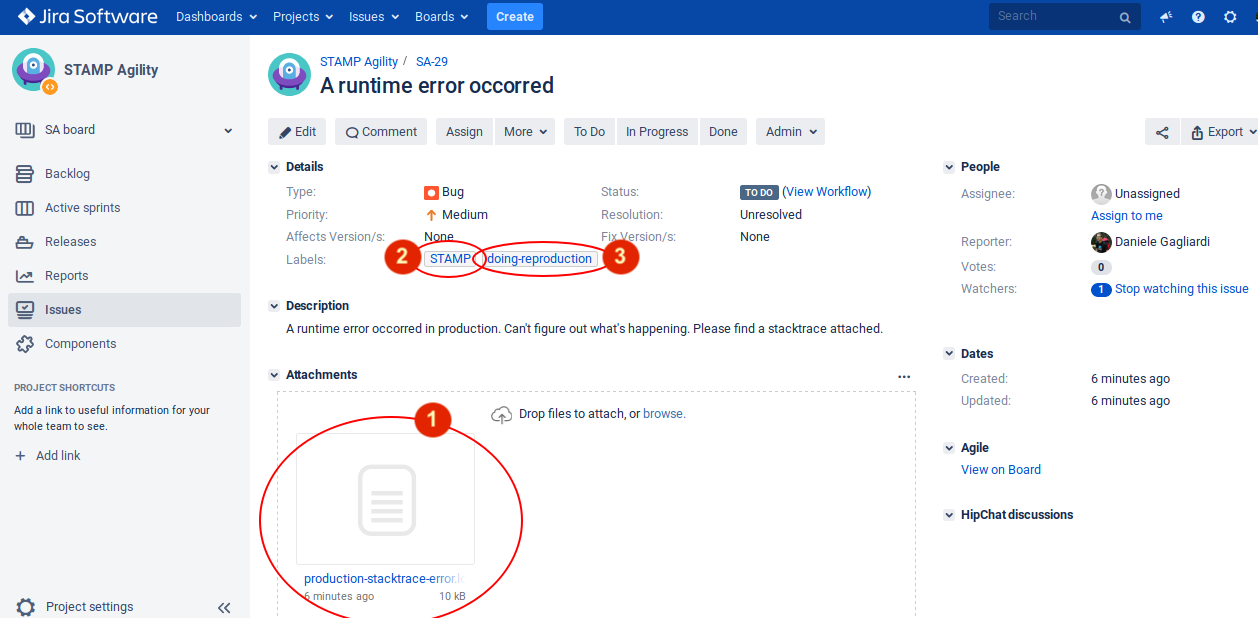
\includegraphics[width=\textwidth]{conclusion/figures/deliverables_wp4_d44_images_jira-doing-reproduction.png}
    \caption{Triggering automatic crash reproduction with \botsing Jira plugin.}
    \label{fig:conclusion:botsingJira1}
\end{figure}

\begin{figure}
    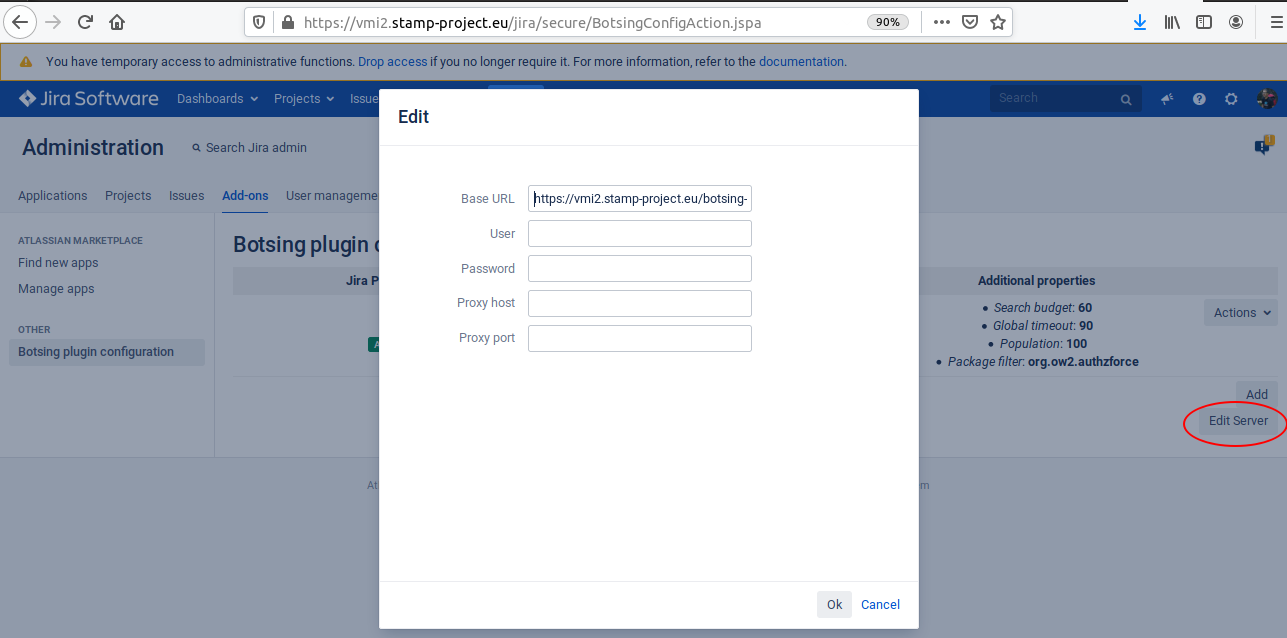
\includegraphics[width=\textwidth]{conclusion/figures/deliverables_wp4_d44_images_jira-botsing-server-configuration.png}
    \caption{\botsing remote server configuration in Jira}
    \label{fig:conclusion:botsingJira2}
\end{figure}


\begin{figure}
    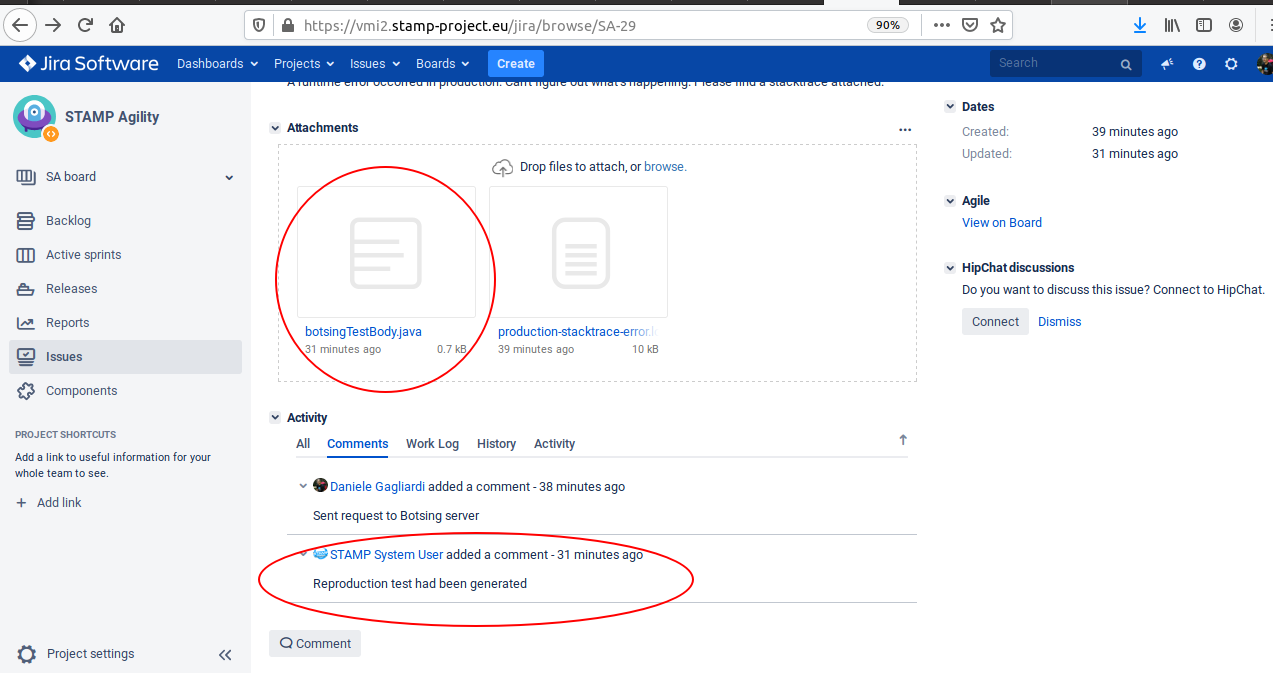
\includegraphics[width=\textwidth]{conclusion/figures/deliverables_wp4_d44_images_jira-reproduction-done.png}
    \caption{crash reproducing test attached to the issue.}
    \label{fig:conclusion:botsingJira3}
\end{figure}


\begin{figure}
    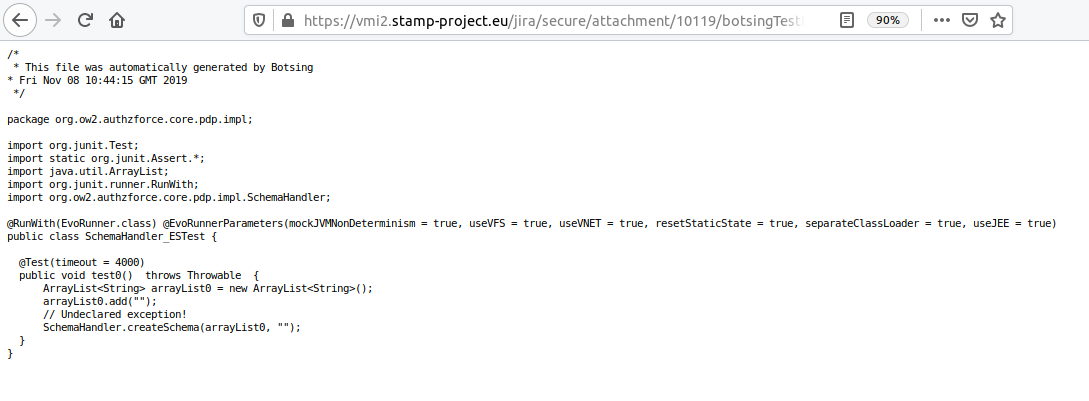
\includegraphics[width=\textwidth]{conclusion/figures/deliverables_wp4_d44_images_jira-generated-test-case.png}
    \caption{A crash reproducing test case bu \botsing Jira plugin.}
    \label{fig:conclusion:botsingJira4}
\end{figure}


\subsection{\cling}

\cling is an open-source class-integration test generation tool for Java. It gets two classes, which are calling each other, and tries to generate tests covering different interactions between these two given classes. Section \ref{sec:cling:results} of this thesis showed that this approach actually managed to detect the integration-level faults. 

Same as \evosuite that has been used widely on industry \cite{almasi2017industrial} for generating unit-level tests, \cling has the potential to be used by different software projects for generating integration-level tests complementing the tests generated by \evosuite. For this reason, we want to implement different plugins for Maven, IntelliJ, and Jenkins to ease the application of \cling on different projects.

\subsection{Commonality Score For Unit Test Generation}
As mentioned in Section \ref{sec:cub:discussion}, we still need to perform a more in-depth investigation about the usefulness of commonality score in finding faults. However, since the introduced secondary objectives, defined according to this metric, aim to change how the statements are covered, we believe they can impact the understandability of the test cases generated by the search process.


\section{Recommendations For Future Work}
This thesis shows that there are still many ways to improve the search-based test generation techniques for various criteria. Hence, this section gives some recommendations for future work.
\subsection{Search-based Crash Reproduction}

\subsubsection{R1: Investigation about improving \CrashFunction}
As described by section \ref{sec:background:evocrash:guidedalg}, \CrashFunction fitness function is used in search-based crash reproduction to measure the distance of each generated test from throwing the same crash as the given one. The three elements in this fitness function may lead to flat landscapes in the search space. For instance, \textbf{the exception coverage} heuristic is a binary value, which indicates whether the same type of exception (as the given one) is thrown or not. Using only 0 and 1 for this heuristic can lead to a flat landscape in the search space.


\subsubsection{R2: Investigation about other secondary and helper objectives}
 Chapters \ref{sec:moho:introduction} and \ref{section:bbc:introduction} show how adding secondary objectives and helper-objectives help the existing \CrashFunction fitness function in reproducing more crashes. However, there are still many possibilities to improce the search objectives. First of all, the \CrashFunction fitness function itself can be modified to make sure that we have less flat landescapes in the search space. Also, more helper objectives can be combined with this fitness function to improve the exploration of the search process.



\subsection{Search-based Integration Testing}
\subsubsection{R3: Search-based test generation for integration of more than two classes}
In Chapter \ref{sec:cling:introduction}, we introduced a new search-based technique for testing interactions between two coupled classes. In the next step, this approach can be extended to handle more classes. It is even possible to design an approach to test the integration of two modules that contain multiple classes.

\subsection{General search-based test generation}
\subsubsection{R4: Using more resources}
This thesis introduced various strategies to utilize the carved information from source code (\eg Chapter \ref{sec:cling:introduction}), existing test cases (\eg Chapter \ref{sec:model_seeding}), and execution logs (Chapter~\ref{sec:cub:intro}) in search-based test generation. However, other resources such as commits addressing previously detected faults can be used to generate more realistic test cases during the search process. Moreover, other useful information can be carved from the application's documentation.

\subsubsection{R5: carving more information}
This thesis used carved information about the method call sequences (\eg Chapters \ref{sec:model_seeding} and \ref{sec:moho:introduction}), call-site information (Chapter \ref{sec:cling:introduction}) and test execution patterns (Chapter \ref{sec:cub:intro}). Other data such as information regarding the input parameters can be carved for white-box search-based test generation to continue this research path. For example, some applications need strings, following a specific grammar and pattern (\eg XML, JSON), to be used in their test generation. These kind of information can be carved from source code and documentations.